\chapter{ Констукторский раздел}
\label{cha:design}
    На рисунке 2.1 представлена схема обычного алгоритма получения среднего геометрического столбцов матрицы (без распараллеливания). На рисунке 2.2 представлена схема варианта распараллеливания алгоритма получения среднего геометрического столбцов матрицы. На риснуке 2.3 показана схема функции, определяющая границы циклов для каждого из потоков.

    \section{Схемы алгоритмов}
    
    
    \begin{figure}[h]
    	\centering
    	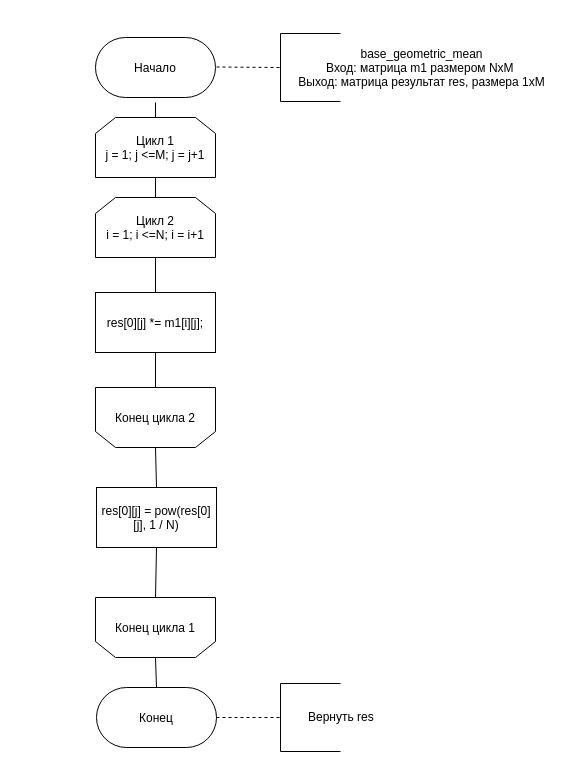
\includegraphics[scale=0.93]{base.jpg}
    	\caption{Схема стандартного алгоритма получения среднего геометрического столбцов матрицы.}
    	\label{fig:mpr}
    \end{figure}
    
    \begin{figure}[h]
    	\centering
    	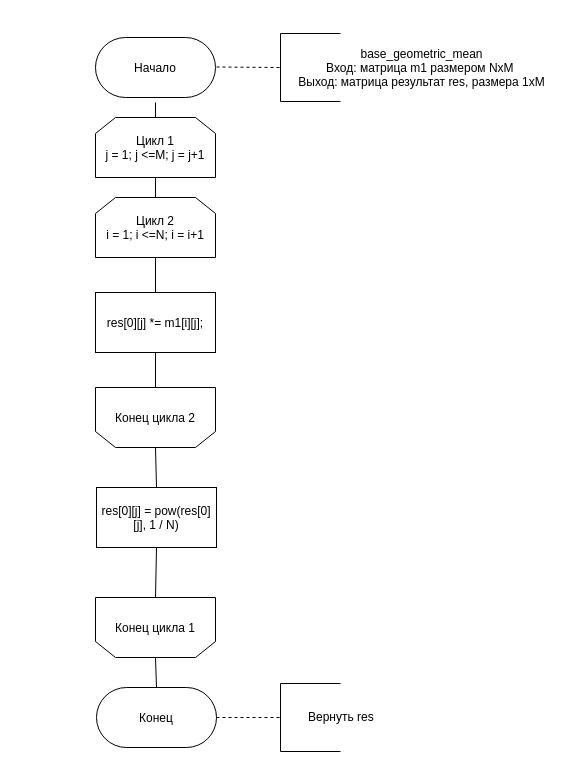
\includegraphics[scale=0.9]{base.jpg}
    	\caption{Схема распараллеленного алгоритма получения среднего геометрического столбцов матрицы.}
    	\label{fig:mpr}
    \end{figure}
    
    \begin{figure}[h]
    	\centering
    	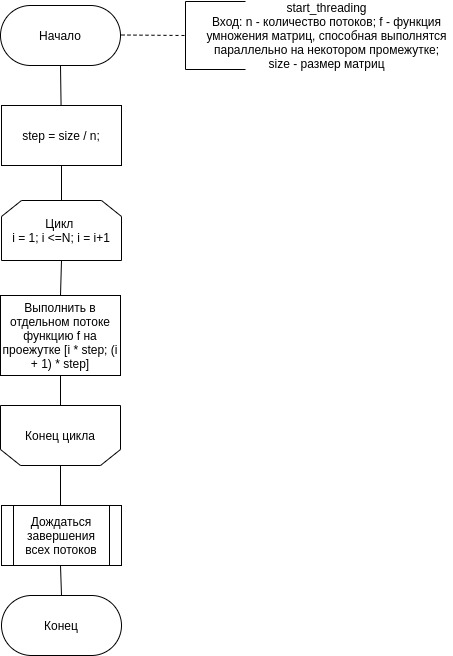
\includegraphics[scale=0.80]{start_threading.jpg}
    	\caption{Функция создания потоков и запуска параллельных реализаций получения среднего геометрического столбцов матрицы}
    	\label{fig:mpr}
    \end{figure}
    
    
    На рисунке 2.4 представленна схема с параллельным выполнением первого цикла
    
    \begin{figure}[h]
    	\centering
    	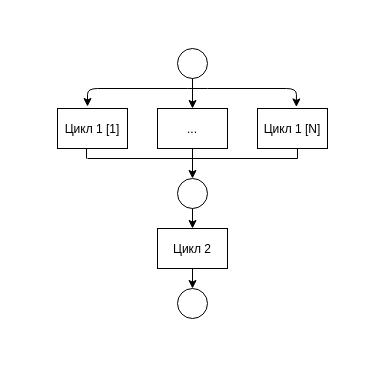
\includegraphics[scale=0.9]{parallel_scheme_01.jpg}
    	\caption{Схема с параллельным выполнением цикла}
    	\label{fig:mpr}
    \end{figure}
    
    
    
    \section{Вывод}
    На основе теоретических данных, полученных из аналитического раздела, была построена схема алгоритма получения среднего геометрического столбцов матрицы, а так же после разделения алгоритма на этапы была предложена схема параллельного выполнения данных этапов.
 

\newpage